\documentclass[aip,cha,reprint,amsmath,amssymb]{revtex4-2}

\usepackage[utf8]{inputenc}
\usepackage[T1]{fontenc}
\usepackage{graphicx}
\usepackage{booktabs}
\usepackage{bm}
\usepackage{xcolor}
\usepackage{hyperref}

\hypersetup{colorlinks=true,linkcolor=blue!70!black,citecolor=blue!70!black,urlcolor=blue!70!black}

\begin{document}

\title{Supplementary Material: Instability, Outlier Amplification, and Positivity Constraints in Next-Generation Reservoir Computing}

\author{Norman Reynaldo Sabill{\'o}n Castro}
\email{sabillonrey2004@gmail.com}
\affiliation{Department of Mathematics, Universidad Nacional Aut{\'o}noma de Honduras, Tegucigalpa, Honduras}

\date{\today}

\maketitle

\noindent This supplement reports three items referenced in the main text: two secondary empirical validation domains (an annual multilateral-lending panel, BCIE, and weekly Honduras retail fuel prices), and a reduced-scale generalization check of the Lorenz63 findings on a second chaotic system (R\"ossler). Both use the same causal protocol audited in the main paper (train/test splits fit exclusively on historical prefix data, a genuine recurrent sparse ESN, and non-negative least squares over a strictly positive feature basis where a positivity requirement applies). Neither domain supports a headline claim on its own: the BCIE result is not statistically significant at the coverage available, and the fuel-price ranking reverses depending on which loss statistic is reported.

% ======================================================================
\section{S1. BCIE Annual Lending Panel: A Non-Significant Secondary Validation}
\label{sec:bcie}
% ======================================================================

The Central American Bank for Economic Integration (BCIE/CABEI) publishes an open panel of loan approvals by member country, 1961--2025. We construct a synthetic systemic hub from the pooled approvals and estimate a coupling operator $\mathbf{P}^*$ via row-wise non-negative least squares under a hub-and-spoke topology mask, comparing four compressions of the NG-RC quadratic feature block (PCA baseline, Ledoit--Wolf shrinkage, Tikhonov-shifted covariance, and direct NNLS regression) against a genuine recurrent sparse ESN reference, under a causal protocol (training through 2019, out-of-sample 2020--2025).

\begin{table}[h]
\centering
\caption{BCIE annual panel, coverage-matched comparison (8 common entities, causal protocol). Diebold--Mariano $p$-values use block-exact resampling by year against the recurrent sparse ESN reference; \texttt{no} indicates the difference is not significant at $\alpha=0.05$.}
\label{tab:bcie}
\begin{ruledtabular}
\begin{tabular}{lrrc}
Method & MASE & $N$ & DM vs.\ ESN ($p$) \\
\midrule
NNLS direct ($k=2$) & \textbf{0.8155} & 32 & 0.50 (no) \\
NNLS direct ($k=3$) & 0.8189 & 32 & 0.50 (no) \\
Recurrent sparse ESN (ref.) & 1.0356 & 32 & -- \\
Tikhonov covariance ($k=3$) & 1.2437 & 28 & 0.75 (no) \\
Ledoit--Wolf ($k=3$) & 1.2437 & 28 & 0.75 (no) \\
Baseline PCA ($k=3$) & 1.2437 & 28 & 0.75 (no) \\
Tikhonov covariance ($k=2$) & 1.3125 & 32 & 0.75 (no) \\
Ledoit--Wolf ($k=2$) & 1.3125 & 32 & 0.75 (no) \\
Baseline PCA ($k=2$) & 1.3125 & 32 & 0.75 (no) \\
\end{tabular}
\end{ruledtabular}
\end{table}

\begin{figure}[h]
\centering

\includegraphics[width=\columnwidth]{figures/fig12_bcie_causal.pdf}
\caption{BCIE annual panel: causal out-of-sample MASE by readout, coverage-matched 8-entity comparison, 2020--2025.}
\label{fig:bcie}
\end{figure}

NNLS direct achieves the lowest point estimate, consistent with the FX/crypto and fuel-price findings that non-negativity constraints tend to help when the target has a structural non-negative nature. However, with only 6 out-of-sample years and 8 common entities, no pairwise Diebold--Mariano comparison reaches significance (all $p \ge 0.50$). We report this as a directionally consistent but statistically inconclusive secondary validation.

% ======================================================================
\section{S2. Honduras Retail Fuel Prices: Ranking Reversals Across Losses}
\label{sec:fuel}
% ======================================================================

We repeat the volatility comparison on 496 weekly observations (2017--2026) of four retail fuel products (Super gasoline, Regular gasoline, Diesel, Kerosene) regulated under Honduras' import-parity pricing system. Here, models predict the \textbf{squared weekly log-returns} ($r_{t+1}^2 = (\log(P_{t+1}/P_t))^2 \ge 0$), evaluated under both QLIKE and MASE.

\begin{table}[h]
\centering
\caption{Honduras fuel squared log-return volatility forecasting, out-of-sample comparison by readout across 496 weeks.}
\label{tab:fuel}
\begin{ruledtabular}
\begin{tabular}{lrrr}
Method & QLIKE & MASE & \% Neg. \\
\midrule
Non-negative NNLS & \textbf{0.359} & 0.485 & 0\% \\
GARCH(1,1) & 0.380 & 0.454 & 0\% \\
GJR-GARCH(1,1) & 0.392 & 0.442 & 0\% \\
Naive persistence & 0.432 & 0.369 & 0\% \\
Legacy OLS (clipped) & 0.542 & 0.587 & 47\% \\
Legacy Ridge (clipped) & 0.552 & 0.734 & 3\% \\
Softplus NG-RC & 0.570 & 0.713 & 0\% \\
EWMA ($\lambda=0.94$) & 0.677 & 0.736 & 0\% \\
Recurrent sparse ESN (log) & 1.313 & \textbf{0.338} & 0\% \\
Log-link Ridge & 1.815 & 0.342 & 0\% \\
\end{tabular}
\end{ruledtabular}
\end{table}

\begin{figure}[h]
\centering

\includegraphics[width=\columnwidth]{figures/fig7_combustibles_precios.pdf}
\caption{Weekly retail prices for four Honduras fuel products, 2017--2026, with shaded windows for COVID-19, hurricanes Eta/Iota, the Russia--Ukraine war, and the 2026 Middle East strait crisis.}
\label{fig:fuel_prices}
\end{figure}

Non-negative NNLS achieves the best QLIKE (0.359), matching the FX/crypto result. But the recurrent sparse ESN achieves the best MASE by a wide margin (0.338, versus 0.485 for NNLS), while ranking near the bottom on QLIKE (1.313). This directly mirrors the median-versus-tail tension: MASE rewards typical-case accuracy, whereas QLIKE punishes rare near-zero predictions severely.

\begin{figure}[h]
\centering

\includegraphics[width=\columnwidth]{figures/fig9_mecanismo_falla_nnls.pdf}
\caption{Mechanism of an NNLS-readout failure case: raw (unclipped) NNLS prediction versus realized volatility for Super and Regular gasoline, illustrating why non-negative weights do not guarantee a non-negative embedding when input features retain signed lags.}
\label{fig:fuel_failure}
\end{figure}

% ======================================================================
\section{S3. Supplementary Figure Reference}
\label{sec:supp_figs}
% ======================================================================

\begin{figure}[h]
\centering
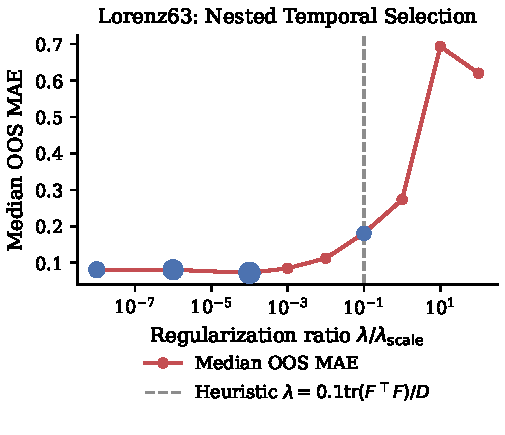
\includegraphics[width=\columnwidth]{figures/fig_supp_lambda_selection.pdf}
\caption{Nested temporal validation path for the Ridge readout's regularization ratio on Lorenz63 (\S3 of the main text), showing the internal holdout MAE across the candidate grid and the ratio selected at each outer window.}
\label{fig:lambda_selection}
\end{figure}

% ======================================================================
\section{S4. Generalization Check: The R\"ossler Attractor}
\label{sec:rossler}
% ======================================================================

To assess whether the three Lorenz63 findings of the main text are specific to that system, we repeat a reduced-scale version of each check on the R\"ossler attractor:
\begin{equation}
\dot x = -y - z, \quad \dot y = x + ay, \quad \dot z = b + z(x-c),
\end{equation}
with standard chaotic parameters $a=b=0.2$, $c=5.7$. R\"ossler's spiral dynamics require coarser subsampling than Lorenz63 ($\Delta t_{\text{feature}}=0.20$ versus Lorenz63's $0.05$). This is a descriptive generalization check, where the multi-step test is evaluated across a single reservoir seed and the noise-filtering test across 5 reservoir seeds (over 30 causal test windows); Ridge is parameterized with the legacy trace heuristic.

\begin{table}[h]
\centering
\caption{R\"ossler descriptive generalization check: all three mechanisms replicate directionally.}
\label{tab:rossler}
\begin{ruledtabular}
\begin{tabular}{lll}
Finding & Lorenz63 & R\"ossler \\
\midrule
$M^4$ log--log slope & 3.99 & 3.79 \\
Multi-step $H{=}10$ median MASE & & \\
\quad Static / ESN (bounded) & 0.43 / 0.74 & 0.26 / 0.58 \\
\quad Legacy Ridge / OLS (unconstrained) & 2.54 / 2.50 & 4.39 / 2.75 \\
Noise-filtering win rate by seed & 100\% (all seeds) & 53\%--67\% (all 5 seeds $>$ 50\%) \\
\end{tabular}
\end{ruledtabular}
\end{table}

\begin{figure}[h]
\centering
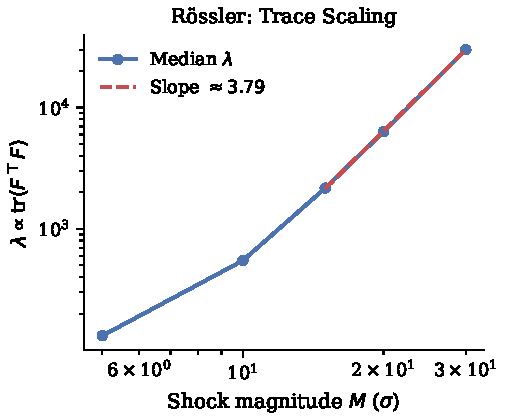
\includegraphics[width=\columnwidth]{figures/fig_rossler_m4.pdf}
\caption{Median trace-proportional $\lambda$ versus shock magnitude $M$ on R\"ossler, log--log scale. The fitted slope (3.79) is close to the Theorem 1 prediction of 4.}
\label{fig:rossler_m4}
\end{figure}

At $H=10$, the unconstrained OLS readout occasionally diverges to MASE exceeding $10^{15}$ under iterated feedback on R\"ossler, starkly illustrating the unconstrained error-compounding mechanism.

\section*{Data and Code Availability}
The data and Python reproduction pipelines supporting this supplement are available in the companion repository and Zenodo archive.

\end{document}
